\documentclass[preprint,12pt]{elsarticle}
\usepackage{amsmath}
\usepackage{booktabs}
\usepackage{graphicx}
\usepackage[colorlinks=true]{hyperref}
\renewcommand{\thesection}{\Roman{section}}
\renewcommand{\thesubsection}{\thesection-\Alph{subsection}}
\graphicspath{{./figs/}}
\begin{document}
\begin{frontmatter}
\title{Multi-Horizon Failure-Risk Models for Battery Failure Prediction: How Much Cross-Chemistry Transfer Is a State-of-Health Shortcut?}
\author{Anonymous}
\address{Affiliation 1, City, Country (e-mail: author1@example.com)}
\begin{abstract}
Predicting whether a lithium-ion cell will fail inside a short operating window matters more for real-time dispatch than remaining-useful-life regression. This study widens a multi-horizon failure-risk classification framework into a validity-focused evaluation covering tree ensembles, a GRU classifier, a discrete-time hazard model, and 60 new Battery Archive cells across six laboratories. Within-dataset discrimination is reliable (fold-mean AUC 0.90--0.96). The central result is a controlled State-of-Health (SOH) ablation: apparent cross-dataset transfer with SOH (pooled AUC up to 1.00) collapses without it, and an unfitted SOH distance rule matches the tuned ensembles. Because SOH enters the failure label and the label window includes the current cycle, with-SOH numbers are diagnostic-proximity upper bounds: prognosis-only evaluation gives 0.838 on Severson. Same-chemistry controls show dataset shift matters at least as much as chemistry. Source-fitted calibration does not transfer, and the ensembles deploy on a \$12 microcontroller in under a millisecond per SRAM-resident model.
\end{abstract}
\begin{keyword}
battery failure prediction \sep state-of-health shortcut \sep cross-dataset transfer \sep probability calibration \sep discrete-time hazard model \sep embedded machine learning
\end{keyword}
\end{frontmatter}

\section{Introduction}
Lithium-ion batteries underpin electrified transport and grids, yet field reliability remains hard to certify. Conventional prognostics casts the problem as remaining-useful-life (RUL) regression \cite{meng2019review,roman2021machine}, which answers a question operators rarely ask in real time: a battery management system needs to know whether a cell survives the next mission, not its aggregate cycle count. Predicting lifetime from field rather than laboratory data remains open \cite{sulzer2021challenge}. Tree ensembles --- Random Forest \cite{breiman2001random}, XGBoost \cite{chen2016xgboost}, LightGBM \cite{ke2017lightgbm} --- serve capacity and RUL estimation, but binary failure-risk classification at multiple horizons is recent \cite{shikdar2026learning}.

Shikdar and Laaksonen \cite{shikdar2026learning} recast the problem as multi-horizon failure-risk classification: for cycle $t$ and horizon $H$, predict whether failure (SOH below 0.80 or voltage sag beyond 6\%) occurs within $H$ cycles. Their gradient boosting model on NASA 18650 (37 LCO cells) reached AUC 0.87--0.90 across $H \in \{10,20,30,50\}$, but left three gaps: one model on one dataset (no learner, hyperparameter, or calibration sensitivity), no cross-dataset check, and no path to the microcontroller where a battery management system runs.

This paper begins from those gaps but is organized around a sharper validity question: \emph{when a failure-risk model appears to transfer between datasets and chemistries, is anything about degradation being transferred, or is the model merely reading a health-state variable that encodes proximity to the failure criterion?} The composite label is defined from SOH, and SOH is also the strongest feature, so a model can score well on transfer while learning only ``distance to the SOH $=$ 0.80 threshold.''

Two adjacent literatures bear on these questions. Transfer learning for battery state estimation is a growing area: Sahoo et al. \cite{sahoo2022transfer} fine-tuned an SOH estimator across NASA and CALCE cells, and Lu et al. \cite{lu2023deep} pretrained on large-scale degradation data; both target SOH regression rather than failure-risk classification, where the horizon-dependent label and shifting calibration add complications. On calibration, Platt scaling \cite{platt1999probabilistic} fits a sigmoid to raw scores while isotonic regression \cite{zadrozny2002transforming} fits a step function; Platt is safer on small datasets \cite{niculescu2005predicting} and imbalanced data \cite{huang2020experimental}, but no prior study compares the two under cross-chemistry shift. A companion study found the calibration layer is the primary point of failure under operating perturbation and that small-sample recalibration largely restores it \cite{shikdar2026robustness}; whether the repair survives cross-chemistry shift is examined here. TreeSHAP \cite{lundberg2020from} is the standard attribution tool for ensembles, edge inference removes latency and connectivity needs \cite{grzesik2024combining}, and online recalibration under shift is an active area \cite{gupta2023online}. Table~\ref{tab:lit} situates this work against these lines of research.

\begin{table}[!t]
\caption{Comparison of Representative Battery Studies With This Work}
\label{tab:lit}
\centering
\footnotesize
\resizebox{\textwidth}{!}{%
\begin{tabular}{lllp{0.38\textwidth}}
\toprule
\textbf{Study} & \textbf{Family} & \textbf{Data} & \textbf{Position relative to this work}\\
\midrule
Meng and Li \cite{meng2019review} & PHM review & Various & Physics-based, data-driven, hybrid families\\
Breiman, Chen, Ke \cite{breiman2001random,chen2016xgboost,ke2017lightgbm} & Tree ensembles & RUL tasks & RUL regression, not failure-risk classification\\
Sahoo et al. \cite{sahoo2022transfer} & Transfer (SOH) & NASA, CALCE & SOH regression only\\
Lu et al. \cite{lu2023deep} & Deep SOH & Large corpora & SOH regression only\\
Platt, Zadrozny et al. \cite{platt1999probabilistic,zadrozny2002transforming,niculescu2005predicting,huang2020experimental} & Calibration & Various & In-domain comparison only\\
Lundberg et al. \cite{lundberg2020from} & Explainability & --- & TreeSHAP for ensembles\\
Grzesik and Mrozek \cite{grzesik2024combining} & Edge ML & --- & No battery failure cases\\
Gupta and Ramdas \cite{gupta2023online} & Online calib.\ & --- & Distribution-shift Platt\\
Shikdar and Laaksonen \cite{shikdar2026learning} & Failure risk & NASA & One model, one dataset (baseline)\\
\textbf{This work} & Failure risk + validity & 8 datasets & Multi-model SOH-shortcut diagnosis, hazard model, edge deployment\\
\bottomrule
\end{tabular}}
\end{table}

The objective of this study is to close the three gaps identified above and, in doing so, to answer the validity question rigorously. The contributions are:
\begin{itemize}
\item a four-model benchmark (three tree ensembles plus a GRU) on two LCO datasets under cell-disjoint splits with cross-fitted, leakage-free calibration;
\item a discrete-time hazard formulation whose survival product is monotone in the horizon by construction, against independent fixed-horizon classifiers that violate monotonicity on 32--45\% of rows (see Supplementary Material);
\item a shortcut diagnosis of cross-dataset transfer: minimal baselines, a factorial feature ablation, a failure-definition ablation relabeling failures by SOH or voltage sag alone, and same-chemistry cross-laboratory controls separating dataset shift from chemistry shift;
\item a cell-as-unit uncertainty treatment: cell-level bootstrap intervals on every headline number, DeLong tests demoted to secondary evidence;
\item calibration analysis under shift with small-sample recalibration, a cost-sensitive operational evaluation, and a complete ESP32-S3 embedded deployment.
\end{itemize}

The remainder of this paper is organized as follows. Section~II describes the methodology, Section~III the results, Section~IV the analysis and limitations, and Section~V concludes.

\section{Methodology}

\subsection{Composite Failure Label}
Following the original protocol \cite{shikdar2026learning}, cell State-of-Health at cycle $k$ is discharge capacity over mean first-10-cycle capacity,
\begin{equation}\label{eq:soh}
\begin{aligned}
\mathrm{SOH}_k^{(c)} &= \frac{Q_k^{(c)}}{\bar{Q}^{(c)}},\\[2pt]
\bar{Q}^{(c)} &= \frac{1}{10}\sum_{i=1}^{10} Q_i^{(c)},
\end{aligned}
\end{equation}
where $Q_k^{(c)}$ is the discharge capacity at cycle $k$. The voltage baseline $\bar{V}^{(c)}$ is defined analogously. A discharge cycle $t$ in cell $c$ is labeled as failing within horizon $H$ if any cycle $k\in[t,t{+}H)$ meets either of two criteria,
\begin{equation}\label{eq:label}
y_t^{(c,H)} \;=\; \begin{cases}
1, & \exists\, k\in[t,t{+}H):\ \mathrm{SOH}_k^{(c)}\le 0.80 \ \text{or}\\[2pt]
& \bar{V}_k^{(c)} < 0.94\,\bar{V}^{(c)},\\[2pt]
0, & \text{otherwise,}
\end{cases}
\end{equation}
and once triggered the label stays 1 for all later cycles. Because the window $[t,t{+}H)$ includes the current cycle, rows scored at or after the failure crossing are labeled positive for every formulation in this paper: with-SOH results therefore mix concurrent failure detection with future failure prediction, and Section~III-C reports the two components separately. This paragraph makes explicit what was already true of every evaluation reported here; the label code is unchanged and no reported number moves as a result of the clarification. The task is to estimate the cumulative failure risk over the horizon,
\begin{equation}\label{eq:risk}
p_t^{(c,H)} \;=\; \Pr\!\bigl(T_f \le t{+}H \mid T_f > t,\ \mathbf{x}_t^{(c)}\bigr),
\end{equation}
where $T_f$ is the failure cycle and $\mathbf{x}_t^{(c)}$ the feature vector at cycle $t$. Datasets without voltage data, or with voltage at the cutoff as in Oxford's flat LFP plateau, fall back to SOH alone.

Three properties of this label definition matter for everything that follows. First, (3) is a fixed-horizon cumulative failure risk, not a discrete-time hazard: each horizon is an independent binary classifier with no monotonicity constraint $p_t^{(c,10)}\le p_t^{(c,20)}\le p_t^{(c,30)}\le p_t^{(c,50)}$. Section~II-G adds a true discrete-time hazard model, and Section~III-H quantifies the violations. Second, the label is \emph{partially defined by SOH itself}, and SOH is also an input feature; a with-SOH model can therefore detect proximity to the SOH $=0.80$ threshold without learning degradation dynamics. Every with-SOH result here is an upper bound including this leakage, and Section~III-F measures it by relabeling failures one endpoint at a time. Third, the endpoints separate: the label can use the SOH criterion alone, voltage sag alone, or both, independently of the feature ablation.

\subsection{Datasets}
Eight public aging datasets are used:
\begin{itemize}
\item \textbf{1) NASA 18650} \cite{saha2007battery}: 37 LCO cells aged under randomized charge--discharge profiles at room temperature, 1~028 cleaned discharge rows in total (about 28 per cell), with diverse failure modes;
\item \textbf{2) CALCE LCO/CX2} \cite{calce2023battery}: 7 cells (CS2\_33--36, CX2\_36--38) at 1C/1C; ambient temperature and discharge duration unlogged;
\item \textbf{3) Oxford} \cite{birkl2017oxford}: 5 LFP pouch cells at 1C/1C; discharge summaries at roughly 100-cycle intervals leave 46--78 usable cycles per cell (320 rows);
\item \textbf{4) MIT--Stanford Severson} \cite{severson2019data,attia2020closedloop}: 141 LFP cells under a fast-charging protocol, 101--2~237 cleaned cycles each (about 117~000 rows in total);
\item \textbf{5) HNEI NMC/LCO} \cite{batteryarchive2023}: 15 NMC/LCO-blend 18650 cells cycled continuously at 25~$^\circ$C under a fixed charge protocol and mixed discharge C-rates, 1016--1064 cycles each --- all reaching the 80\% SOH end-of-life criterion;
\item \textbf{6) SNL NCA} \cite{batteryarchive2023,preger2020degradation}: 18 NCA cells at 15--35~$^\circ$C, 451--904 cycles each;
\item \textbf{7) SNL NMC} \cite{batteryarchive2023,preger2020degradation}: 6 NMC 18650 cells at 15--25~$^\circ$C, 384--670 cycles each;
\item \textbf{8) SNL LFP} \cite{batteryarchive2023,preger2020degradation}: 21 LFP cells at 15--35~$^\circ$C, 3022--4544 cycles each (5 reach 80\% SOH).
\end{itemize}
Items 5--8 are the Battery Archive ``Cycle Test Data'' export \cite{batteryarchive2023} (September 2026 summaries; SNL matrix per Preger et al.~\cite{preger2020degradation}), used only as \emph{transfer targets} and within-group controls.

A pre-registered cleaning rule admits a cell only if it passes formation-cycle removal, Hampel despiking of the capacity trace, truncation at sustained level shifts, per-cycle voltage validity, and a minimum of 20 usable cycles. Of 75 downloaded cells, 60 pass (15 + 6 NMC, 18 NCA, 21 LFP; 106\,787 cycle rows); the remaining 15 are excluded --- all 15 for mixed state-of-charge windows --- and are never used. On every admitted cell the SOH end-of-life crossing occurs no later than the voltage-sag crossing, so the composite label on the new groups is, in effect, the SOH criterion alone.

One consequence of the Oxford logging resolution deserves emphasis. Consecutive cleaned cycles are roughly 100 cycles apart, so every horizon $H\in\{10,20,30,50\}$ is shorter than the sampling interval and the positive-label rows are \emph{identical for all four horizons}: Oxford measures pooled failure detection, not horizon-resolved prediction, and its per-cell means rest effectively on four cells (Cell5 contributes one positive row). Both caveats apply to every Oxford number in this paper.

\subsection{Features and Preprocessing}
Each cycle is described by seven scalar features: cycle index, average and minimum discharge voltage, average discharge current, average temperature, discharge duration, and SOH. Trees are scale-invariant and need no standardization; the GRU and logistic baselines are standardized with training-set statistics. Unlogged CALCE and Battery Archive columns (temperature, duration, current) are zero-filled; a constant-zero column cannot split within one dataset but acts as a dataset identifier in pooled training, a confound Section~III-G controls with a common-feature subset.

\subsection{Tree Models and Hyperparameters}
Three tree ensembles are benchmarked with hyperparameters matched to the original study \cite{shikdar2026learning}: XGBoost \cite{chen2016xgboost} with max\_depth 4, 300 estimators, learning rate 0.05, subsample 0.8, colsample\_bytree 0.8, and min\_child\_weight 5; LightGBM \cite{ke2017lightgbm} with the same depth, count, and rate; and Random Forest \cite{breiman2001random} with max\_depth 6 and 300 estimators. All use random\_state 42 for deterministic replication.

\subsection{GRU Sequence Classifier}
A compact GRU tests whether sequence-aware representations transfer across chemistries. It ingests sliding windows of $W{=}10$ cycles per cell through one 8-unit GRU layer,
\begin{equation}\label{eq:gru}
\begin{aligned}
\mathbf{r}_t &= \sigma(W_r\mathbf{x}_t + U_r\mathbf{h}_{t-1}),\\[2pt]
\mathbf{z}_t &= \sigma(W_z\mathbf{x}_t + U_z\mathbf{h}_{t-1}),\\[2pt]
\tilde{\mathbf{h}}_t &= \tanh(W_h\mathbf{x}_t + U_h(\mathbf{r}_t\odot\mathbf{h}_{t-1})),\\[2pt]
\mathbf{h}_t &= (1-\mathbf{z}_t)\odot\mathbf{h}_{t-1} + \mathbf{z}_t\odot\tilde{\mathbf{h}}_t,
\end{aligned}
\end{equation}
and the final hidden state maps through a sigmoid linear layer to the failure probability (Adam, learning rate 0.005, binary cross-entropy). The 8-unit width matches the small training-cell counts. For cross-dataset runs the feature set is reduced to the common, unit-safe set --- cycle number, average and minimum voltage, plus SOH when enabled --- standardized with training-set statistics; current, temperature, and duration are dropped for unit safety. The trees are evaluated on the identical common set (Section~III-C), so no architecture claim rests on a feature-confounded comparison.

\subsection{Minimal Baselines}
Because the central question is whether apparent performance is a health-state shortcut, the most important models are embarrassingly simple ones \cite{shikdar2026learning}:
\begin{itemize}
\item \textbf{SOH distance rule}: the fitted-free score $d_t = 0.80 - \mathrm{SOH}_t$, i.e., distance below the label threshold;
\item \textbf{SOH-only} logistic regression, $\Pr(y_t^{(H)}{=}1)=\sigma(a_H\,\mathrm{SOH}_t+b_H)$;
\item \textbf{cycle-only} logistic regression on the cycle index;
\item \textbf{SOH + cycle} logistic regression;
\item \textbf{sensors-only} logistic regression on the five non-SOH, non-cycle features;
\item \textbf{full-feature} logistic regression on all seven features.
\end{itemize}
If the SOH-only and distance-rule baselines reproduce most of the transferable performance of the tuned ensembles, then the ensembles contribute little beyond reading the health state --- the negative result this validity analysis predicts.

\subsection{A True Discrete-Time Hazard Model}
To complement the four independent fixed-horizon classifiers, we also fit an explicit discrete-time survival model. For each observed cycle $t$ and offset $\ell\in\{1,\dots,L\}$ with $L{=}50$, define the hazard
\begin{equation}\label{eq:hazard}
h_\ell(t) \;=\; \Pr\!\bigl(T_f = t{+}\ell \mid T_f \ge t{+}\ell,\ \mathbf{x}_t\bigr),
\end{equation}
conditional on the features measured at $t$ only. One pooled classifier --- XGBoost, and a logistic regression --- is fit on the offset-expanded at-risk rows $(\mathbf{x}_t, \ell)$ with target $\mathbf{1}\{T_f = t{+}\ell\}$, restricted to $t{+}\ell \le T_f$, with $\ell$ as an input feature. The cumulative risk over horizon $H$ is the survival product
\begin{equation}\label{eq:survival}
R(t,H) \;=\; 1 - \prod_{\ell=1}^{H}\bigl(1-\hat h_\ell(t)\bigr),
\end{equation}
which is monotone non-decreasing in $H$ by construction and yields all four horizons from one model. Rows at or after failure are scored exactly like the fixed-horizon classifiers score them, so the evaluation rows are identical across formulations.

\subsection{Calibration Protocol}
Three post-hoc calibration schemes are compared: Platt scaling fits a sigmoid to the raw scores $s_i$,
\begin{equation}\label{eq:platt}
p_i \;=\; \frac{1}{1+\exp(-\alpha s_i - \beta)},
\end{equation}
by logistic regression; isotonic regression \cite{zadrozny2002transforming} fits the non-decreasing step function that minimizes squared error, implemented with scikit-learn's \texttt{IsotonicRegression} and out-of-bounds clipping; and temperature scaling divides the logit of the score by a single fitted temperature.

The protocol is leakage-clean. For every within-dataset fold, calibrators are fitted on \emph{cross-fitted out-of-fold scores} from an inner cell-disjoint GroupKFold over the training cells; untouched test cells are scored by a model trained on all training cells. In transfer, calibrators are fitted on source out-of-fold scores only. No calibrator is ever fitted on the scores it is applied to, and no test cell contributes to training or calibration.

A reproducibility note is retained from the original study comparison. The original study \cite{shikdar2026learning} reported Brier scores around 0.032; re-execution yields roughly 0.09--0.29, a gap of unknown cause that does not affect the relative comparisons forming the core of this paper.

\subsection{Transfer Protocols}
Transfer is evaluated by training on LCO cells (NASA alone, CALCE alone, or both) and testing on the target cells. Performance is reported per cell and pooled with cell-level bootstrap intervals; pooling alone can hide degenerate constant-score behavior, which per-cell statistics expose. Three families of transfer are used:

\begin{itemize}
\item \textbf{Cross-chemistry} (LCO$\to$LFP): NASA, CALCE, or both $\to$ Oxford and $\to$ Severson, with and without SOH, and on the common feature set shared with the GRU;
\item \textbf{Same-chemistry, cross-laboratory controls}: NASA$\to$CALCE and CALCE$\to$NASA (LCO$\to$LCO) and Severson$\to$Oxford and Oxford$\to$Severson (LFP$\to$LFP). Chemistry, laboratory, protocol, and logging all change at once between any source and target, so ``cross-chemistry'' is shorthand for cross-\emph{dataset} shifts, and these controls separate the two;
\item \textbf{Feature-definition ablations}: the factorial feature grid of Section~III-E and the failure-endpoint relabeling of Section~III-F.
\end{itemize}

\subsection{Evaluation and Statistical Testing}
\label{sec:eval}
Within-dataset evaluation uses 5-fold cell-grouped cross-validation on NASA (37 cells) and leave-one-cell-out on CALCE (7 cells): splits are cell-disjoint, models retrained per horizon. The experimental unit is the cell: headline AUCs are fold means with fold SDs, every headline carries a 95\% cell-resampling interval (2~000 draws, 400 for Severson), and paired comparisons reuse the same resamples.

The DeLong nonparametric test \cite{delong1988comparing} for paired ROC curves is retained as secondary evidence. It treats every cycle-level prediction as independent; because cycles within a cell are correlated, its $p$-values are inflated by pseudoreplication and are read only as directional consistency checks, never as precise significance statements.

Discrimination alone is not enough for a reliability-oriented study, so each within-dataset configuration also reports the Brier score, expected calibration error (10 equal-width bins), log loss, the slope and intercept of a logistic recalibration of the predicted probabilities (slope 1 and intercept 0 indicate perfect calibration), the area under the precision--recall curve, which is sensitive to the horizon-dependent class prevalence that AUC ignores, and sensitivity at a fixed 10\% false-positive rate. Operational, cost-sensitive evaluation is described with the results in Section~III-K.

Three reporting conventions apply throughout. Pooled AUC is dominated by long-lived cells, so per-cell statistics and cell-level bootstrap intervals are the primary evidence. Failure prevalence rises with the horizon, so Brier score, calibration error, thresholds, and precision--recall are horizon-dependent. The cost model prices a missed failure at 20 times a false alarm; thresholds use a 10\% source false-alarm budget, and sensitivity to other budgets is untested.

\subsection{Embedded Deployment Architecture}
The deployment pipeline exports the three trained models into one flat binary run on an ESP32-S3 by a hand-written C tree walker: a 12-byte header, a $3{\times}4$-byte offset table, and per-model sections of consecutive node arrays (split feature, float threshold, child indices; leaves store class-1 probabilities). Writing $\ell_t$ for the leaf value reached in tree $t$ and $T$ for the number of trees, Random Forest averages and clamps its leaf probabilities,
\begin{equation}\label{eq:rf}
p \;=\; \mathrm{clamp}\!\left(\frac{1}{T}\sum_{t=1}^{T}\ell_t,\ 0,\ 1\right),
\end{equation}
while XGBoost and LightGBM pass the summed score through a sigmoid,
\begin{equation}\label{eq:sigmoid}
p \;=\; \frac{1}{1+\exp\!\bigl(-\textstyle\sum_{t=1}^{T}\ell_t - s_0\bigr)},
\end{equation}
where $s_0$ is the model's initialization score ($s_0\neq 0$ only for XGBoost). Correctness is confirmed in three stages --- a Python walker mirroring the C logic against \texttt{predict\_proba()}, a cross-compiled x86\_64 binary, and on-target ESP32-S3 execution --- all below $10^{-5}$ maximum absolute error before deployment is accepted.
\section{Results}

\subsection{Within-Dataset Performance}
Table~\ref{tab:within} summarizes within-dataset performance as fold-mean AUC $\pm$ SD under the leakage-clean protocol (LOCO on CALCE, 5-fold grouped CV on NASA), with Platt Brier scores. Every tree configuration clears 0.89 at every horizon on both datasets (Fig.~\ref{fig:within}); the GRU matches the means with higher fold variance, and the single-fit hazard model lands in the same range. On the four new Battery Archive groups, 38 of 39 tree--group--horizon configurations reach 0.85, spanning 0.61--1.00 --- though the mostly-censored LFP-SNL group (0.031 prevalence) is supporting evidence only.

\begin{table}[!t]
\caption{Within-Dataset Failure-Risk Performance Across Four Horizons (Fold-Mean AUC $\pm$ Fold SD; Tree Ensembles and GRU Platt-Calibrated, Hazard Models Raw; CALCE Uses Leave-One-Cell-Out, NASA 5-Fold Cell-Grouped CV). Brier Is the Platt Pooled Value Averaged Over Horizons (Raw for Hazard Rows).}
\label{tab:within}
\centering
\resizebox{\textwidth}{!}{%
\begin{tabular}{llcccccc}
\toprule
\textbf{Model} & \textbf{Dataset} & \textbf{H=10} & \textbf{H=20} & \textbf{H=30} & \textbf{H=50} & \textbf{Mean AUC} & \textbf{Brier}\\
\midrule
XGBoost & NASA & 0.903$\pm$0.097 & 0.899$\pm$0.121 & 0.910$\pm$0.111 & 0.918$\pm$0.115 & 0.907 & 0.182 \\
LightGBM & NASA & 0.912$\pm$0.065 & 0.909$\pm$0.126 & 0.892$\pm$0.121 & 0.901$\pm$0.073 & 0.903 & 0.206 \\
Random Forest & NASA & 0.911$\pm$0.106 & 0.901$\pm$0.109 & 0.912$\pm$0.113 & 0.927$\pm$0.107 & 0.913 & 0.201 \\
GRU & NASA & 0.872$\pm$0.122 & 0.893$\pm$0.114 & 0.884$\pm$0.083 & 0.856$\pm$0.128 & 0.876 & 0.307 \\
Hazard XGBoost & NASA & 0.918$\pm$0.086 & 0.935$\pm$0.086 & 0.937$\pm$0.081 & 0.927$\pm$0.070 & 0.929 & 0.182 \\
Hazard Logistic & NASA & 0.902$\pm$0.064 & 0.899$\pm$0.057 & 0.896$\pm$0.045 & 0.867$\pm$0.052 & 0.891 & 0.175 \\
XGBoost & CALCE & 0.965$\pm$0.041 & 0.967$\pm$0.036 & 0.967$\pm$0.040 & 0.943$\pm$0.071 & 0.961 & 0.075 \\
LightGBM & CALCE & 0.967$\pm$0.047 & 0.968$\pm$0.038 & 0.943$\pm$0.070 & 0.942$\pm$0.076 & 0.955 & 0.075 \\
Random Forest & CALCE & 0.934$\pm$0.074 & 0.933$\pm$0.070 & 0.917$\pm$0.098 & 0.903$\pm$0.110 & 0.922 & 0.070 \\
GRU & CALCE & 0.952$\pm$0.072 & 0.959$\pm$0.083 & 0.935$\pm$0.090 & 0.921$\pm$0.090 & 0.942 & 0.130 \\
Hazard XGBoost & CALCE & 0.894$\pm$0.135 & 0.893$\pm$0.130 & 0.916$\pm$0.095 & 0.889$\pm$0.096 & 0.898 & 0.108 \\
Hazard Logistic & CALCE & 0.979$\pm$0.042 & 0.948$\pm$0.119 & 0.936$\pm$0.138 & 0.945$\pm$0.117 & 0.952 & 0.122 \\
\bottomrule
\end{tabular}}
\end{table}

\begin{figure}[!t]
\centering
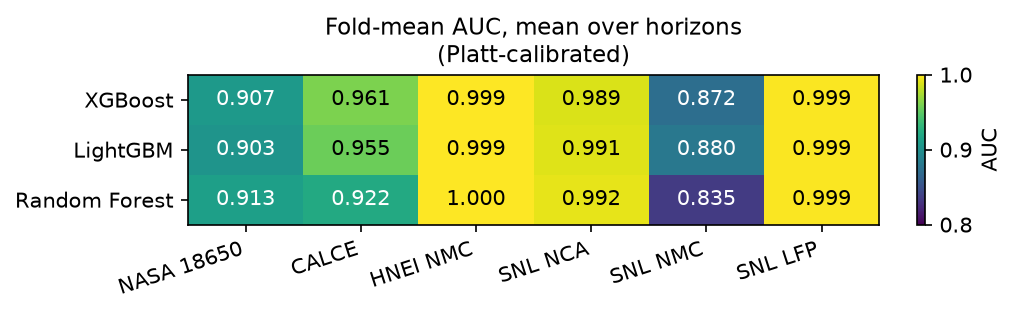
\includegraphics[width=1.0\textwidth]{Fig01_Within_Dataset_AUC.png}
\caption{Within-dataset AUC heatmap for the tree ensembles, mean across horizons, Platt-calibrated. Right block: the four new Battery Archive groups. GRU and hazard within-dataset numbers are in Table~\ref{tab:within}.}
\label{fig:within}
\end{figure}

\subsection{Calibration Under Cross-Fitting}
Calibration is fitted leakage-clean on cross-fitted out-of-fold scores. Raw scores rank best within dataset; isotonic's tied step outputs destroy precision--recall (NASA PR-AUC 0.77 raw versus 0.64 isotonic) while temperature scaling is most balanced on NASA and Platt on CALCE calibration error. The full comparison is in the Supplementary Material.
\subsection{Cross-Dataset Transfer With and Without SOH}
Table~\ref{tab:crosswith} reports LCO$\to$LFP transfer at $H{=}20$ with SOH kept, and Table~\ref{tab:crossno} without; Fig.~\ref{fig:collapse} maps the AUC drop from removing SOH. Every number carries a cell-level bootstrap interval plus per-cell mean and standard deviation. With SOH, the trees reach pooled raw AUC up to 1.00 (Oxford) and 0.90 (Severson). Without SOH, transfer collapses to at most 0.58 on Oxford and 0.53--0.75 on Severson --- point estimates fall below 0.5 in several configurations, significantly so only for the hazard model on Oxford.

The GRU shows a source-dependent instability at three seeds: per-cell AUC on Severson without SOH is $0.987\pm0.015$ for NASA (stable, near-oracle) but $0.479\pm0.451$ for CALCE (seeds 0.21--1.00) and $0.893\pm0.131$ pooled --- against $0.998\pm0.003$, $0.964\pm0.033$ and $0.991\pm0.015$ with SOH. On the identical common feature set the trees retain their table~\ref{tab:crosswith} behavior, so the gap is architectural, not featural. On Oxford the GRU is at or below chance (see Supplementary Material).

\begin{table}[!t]
\caption{Cross-Dataset Transfer at H=20 With SOH (Upper-Bound / Label-Proximity Regime). Raw-Score Pooled AUC With Cell-Level Bootstrap 95\% CI; Per-Cell Mean $\pm$ SD Across Test Cells (Oxford: Five Cells, One With a Single Positive Row; See Section II-B).}
\label{tab:crosswith}
\centering
\resizebox{\textwidth}{!}{%
\begin{tabular}{llcccc}
\toprule
 & & \multicolumn{2}{c}{\textbf{Oxford}} & \multicolumn{2}{c}{\textbf{Severson}}\\
\cmidrule(lr){3-4}\cmidrule(l){5-6}
\textbf{Training} & \textbf{Model} & \textbf{Pooled AUC [CI]} & \textbf{Per-cell} & \textbf{Pooled AUC [CI]} & \textbf{Per-cell}\\
\midrule
NASA & XGBoost & 0.957 [0.931,\,0.987] & 0.959$\pm$0.037 & 0.871 [0.767,\,0.997] & 0.997$\pm$0.010 \\
NASA & LightGBM & 1.000 [1.000,\,1.000] & 1.000$\pm$0.000 & 0.849 [0.724,\,0.998] & 0.992$\pm$0.048 \\
NASA & Random Forest & 1.000 [1.000,\,1.000] & 1.000$\pm$0.000 & 0.861 [0.739,\,0.998] & 0.999$\pm$0.007 \\
CALCE & XGBoost & 0.850 [0.764,\,0.910] & 0.763$\pm$0.245 & 0.850 [0.749,\,0.967] & 0.957$\pm$0.054 \\
CALCE & LightGBM & 0.889 [0.827,\,0.932] & 0.837$\pm$0.193 & 0.863 [0.782,\,0.957] & 0.952$\pm$0.037 \\
CALCE & Random Forest & 0.850 [0.773,\,0.899] & 0.766$\pm$0.169 & 0.902 [0.834,\,0.984] & 0.996$\pm$0.022 \\
ALL LCO & XGBoost & 0.917 [0.878,\,0.965] & 0.826$\pm$0.265 & 0.896 [0.812,\,0.995] & 0.995$\pm$0.015 \\
ALL LCO & LightGBM & 0.971 [0.959,\,0.981] & 0.969$\pm$0.015 & 0.882 [0.789,\,0.990] & 0.993$\pm$0.026 \\
ALL LCO & Random Forest & 0.989 [0.979,\,0.998] & 0.992$\pm$0.013 & 0.889 [0.796,\,0.998] & 0.996$\pm$0.021 \\
\bottomrule
\end{tabular}}
\end{table}

\begin{table}[!t]
\caption{Cross-Dataset Transfer at H=20 Without SOH (Prognostically Meaningful Regime). Columns as in Table~\ref{tab:crosswith}.}
\label{tab:crossno}
\centering
\resizebox{\textwidth}{!}{%
\begin{tabular}{llcccc}
\toprule
 & & \multicolumn{2}{c}{\textbf{Oxford}} & \multicolumn{2}{c}{\textbf{Severson}}\\
\cmidrule(lr){3-4}\cmidrule(l){5-6}
\textbf{Training} & \textbf{Model} & \textbf{Pooled AUC [CI]} & \textbf{Per-cell} & \textbf{Pooled AUC [CI]} & \textbf{Per-cell}\\
\midrule
NASA & XGBoost & 0.518 [0.513,\,0.522] & 0.519$\pm$0.006 & 0.595 [0.510,\,0.726] & 0.676$\pm$0.184 \\
NASA & LightGBM & 0.533 [0.497,\,0.543] & 0.448$\pm$0.201 & 0.527 [0.422,\,0.672] & 0.535$\pm$0.183 \\
NASA & Random Forest & 0.521 [0.487,\,0.537] & 0.442$\pm$0.198 & 0.674 [0.561,\,0.826] & 0.836$\pm$0.176 \\
CALCE & XGBoost & 0.416 [0.264,\,0.554] & 0.360$\pm$0.208 & 0.682 [0.670,\,0.695] & 0.806$\pm$0.082 \\
CALCE & LightGBM & 0.462 [0.307,\,0.579] & 0.410$\pm$0.207 & 0.643 [0.530,\,0.721] & 0.830$\pm$0.042 \\
CALCE & Random Forest & 0.501 [0.320,\,0.641] & 0.435$\pm$0.243 & 0.665 [0.547,\,0.749] & 0.870$\pm$0.049 \\
ALL LCO & XGBoost & 0.429 [0.279,\,0.597] & 0.415$\pm$0.240 & 0.750 [0.692,\,0.835] & 0.860$\pm$0.139 \\
ALL LCO & LightGBM & 0.332 [0.112,\,0.515] & 0.316$\pm$0.209 & 0.718 [0.634,\,0.850] & 0.808$\pm$0.167 \\
ALL LCO & Random Forest & 0.581 [0.516,\,0.644] & 0.608$\pm$0.103 & 0.746 [0.673,\,0.845] & 0.876$\pm$0.115 \\
\bottomrule
\end{tabular}}
\end{table}

\begin{figure}[!t]
\centering
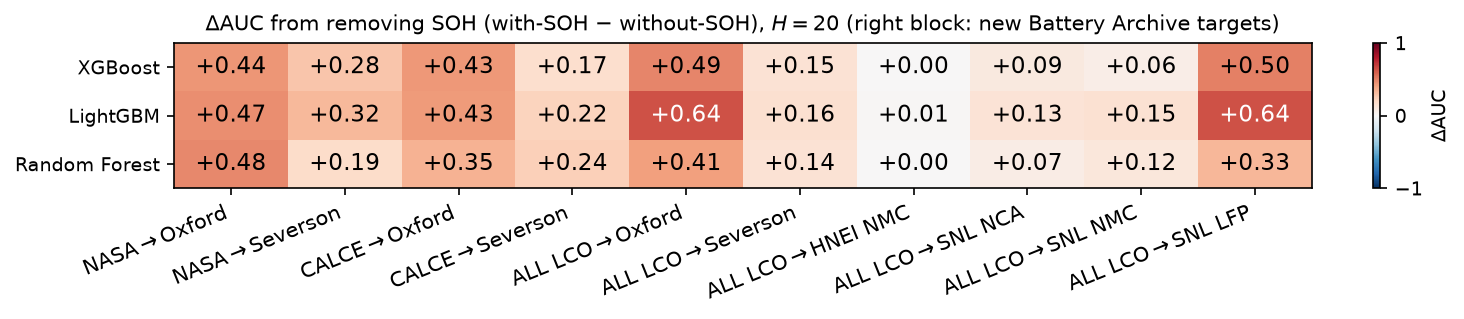
\includegraphics[width=0.95\textwidth]{fig_collapse_map.png}
\caption{Transferability collapse map at $H{=}20$ for the tree ensembles: the AUC drop from removing SOH, per source$\to$target pair and model. Positive values mean SOH removal destroys apparent transfer performance; the near-uniform saturation at the maximum drop is the signature of a single-feature shortcut rather than of distributed degradation knowledge. Right block: ALL-LCO $\to$ new Battery Archive targets. GRU deltas are reported in the text.}
\label{fig:collapse}
\end{figure}



The reading that survives the uncertainty treatment is deliberately modest. SOH appears on both sides of the learning problem --- in the feature vector and inside the label definition --- so high with-SOH transfer is compatible with two mechanisms: a chemistry-dependent mapping from SOH to remaining life, and mere detection of proximity to the SOH $=0.80$ criterion that defines the label. The experiments that follow separate these mechanisms.

Diagnosis or prognosis? Because the label window includes the scoring cycle, rows from already-failed cells score positive. Table~\ref{tab:prog} splits headline transfer numbers into all-rows AUC and prognosis-only AUC on the same scores restricted to rows with SOH still above 0.80. On Severson at $H{=}20$, XGBoost with SOH moves from 0.896 to 0.838 [0.760, 0.991] and without SOH from 0.750 to 0.721 [0.666, 0.833]: 99\% of rows are scored above threshold, so concurrent detection explains only about 0.05--0.07 there; the rest is near-threshold ranking, priced by the failure-definition ablation in Section~III-F. The distance rule behaves identically (0.912 to 0.862). On the new targets the diagnostic share is larger wherever cells linger below threshold --- HNEI 0.993 to 0.963 (28% above), NCA 0.972 to 0.886 (63% above), NMC-SNL 0.772 to 0.729 (60% above), LFP-SNL 0.998 to 0.991 (97% above). The split is conservative --- rows just above 0.80 still count as prognosis --- so no with-SOH number here is pure prognosis: all are diagnostic-proximity upper bounds.

\begin{table}[!t]
\caption{Diagnosis Versus Prognosis at H=20 (ALL-LCO Source, Raw Scores): All-Rows Pooled AUC [Cell-Level CI Where Computed] Against Prognosis-Only AUC on Rows Scored While SOH$>$0.80, With the Share of Rows Scored Above Threshold. GRU and Distance-Rule Rows Are Point Estimates.}
\label{tab:prog}
\centering
\resizebox{\textwidth}{!}{%
\begin{tabular}{lllccc}
\toprule
\textbf{Target} & \textbf{Model} & \textbf{Features} & \textbf{All rows} & \textbf{Prognosis-only} & \textbf{Frac.\ above}\\
\midrule
Severson & GRU & common, no SOH & 0.631  & 0.553  & 0.99 \\
Severson & GRU & common+SOH & 0.827  & 0.756  & 0.99 \\
Severson & LightGBM & no SOH & 0.718 [0.634,0.846] & 0.674 [0.597,0.851] & 0.99 \\
Severson & LightGBM & with SOH & 0.882 [0.786,0.990] & 0.814 [0.732,0.978] & 0.99 \\
Severson & SOH-dist rule & dist rule & 0.912  & 0.862  & 0.99 \\
Severson & SOH-dist rule & SOH-only & 0.912  & 0.862  & 0.99 \\
Severson & Random Forest & no SOH & 0.746 [0.673,0.845] & 0.705 [0.632,0.843] & 0.99 \\
Severson & Random Forest & with SOH & 0.889 [0.783,0.998] & 0.825 [0.737,0.996] & 0.99 \\
Severson & XGBoost & no SOH & 0.750 [0.692,0.835] & 0.721 [0.666,0.833] & 0.99 \\
Severson & XGBoost & with SOH & 0.896 [0.804,0.995] & 0.838 [0.760,0.991] & 0.99 \\
HNEI NMC & LightGBM & no SOH & 0.988 [0.974,0.996] & 0.905 [0.863,0.944] & 0.28 \\
HNEI NMC & LightGBM & with SOH & 0.999 [0.998,0.999] & 0.969 [0.946,0.987] & 0.28 \\
HNEI NMC & Random Forest & no SOH & 0.996 [0.994,0.999] & 0.945 [0.908,0.978] & 0.28 \\
HNEI NMC & Random Forest & with SOH & 0.999 [0.999,1.000] & 0.981 [0.970,0.993] & 0.28 \\
HNEI NMC & XGBoost & no SOH & 0.989 [0.977,0.997] & 0.908 [0.870,0.945] & 0.28 \\
HNEI NMC & XGBoost & with SOH & 0.993 [0.983,0.999] & 0.963 [0.935,0.987] & 0.28 \\
SNL NCA & LightGBM & no SOH & 0.850 [0.791,0.911] & 0.841 [0.798,0.889] & 0.63 \\
SNL NCA & LightGBM & with SOH & 0.985 [0.974,0.993] & 0.891 [0.845,0.946] & 0.63 \\
SNL NCA & Random Forest & no SOH & 0.911 [0.875,0.951] & 0.837 [0.779,0.907] & 0.63 \\
SNL NCA & Random Forest & with SOH & 0.983 [0.974,0.992] & 0.901 [0.858,0.957] & 0.63 \\
SNL NCA & XGBoost & no SOH & 0.878 [0.824,0.930] & 0.849 [0.803,0.895] & 0.63 \\
SNL NCA & XGBoost & with SOH & 0.972 [0.956,0.988] & 0.886 [0.837,0.943] & 0.63 \\
SNL NMC & LightGBM & no SOH & 0.693 [0.570,0.959] & 0.728 [0.577,0.956] & 0.60 \\
SNL NMC & LightGBM & with SOH & 0.847 [0.743,0.982] & 0.722 [0.604,0.956] & 0.60 \\
SNL NMC & Random Forest & no SOH & 0.742 [0.689,0.874] & 0.649 [0.604,0.793] & 0.60 \\
SNL NMC & Random Forest & with SOH & 0.858 [0.748,0.975] & 0.706 [0.613,0.929] & 0.60 \\
SNL NMC & XGBoost & no SOH & 0.709 [0.612,0.953] & 0.730 [0.599,0.946] & 0.60 \\
SNL NMC & XGBoost & with SOH & 0.772 [0.677,0.979] & 0.729 [0.608,0.960] & 0.60 \\
SNL LFP & LightGBM & no SOH & 0.359 [0.282,0.443] & 0.383 [0.311,0.467] & 0.97 \\
SNL LFP & LightGBM & with SOH & 0.999 [0.998,1.000] & 0.993 [0.988,0.998] & 0.97 \\
SNL LFP & Random Forest & no SOH & 0.666 [0.569,0.769] & 0.588 [0.565,0.616] & 0.97 \\
SNL LFP & Random Forest & with SOH & 0.999 [0.998,1.000] & 0.994 [0.990,0.999] & 0.97 \\
SNL LFP & XGBoost & no SOH & 0.496 [0.455,0.531] & 0.517 [0.481,0.575] & 0.97 \\
SNL LFP & XGBoost & with SOH & 0.998 [0.997,1.000] & 0.991 [0.985,0.997] & 0.97 \\
\bottomrule
\end{tabular}}
\end{table}

\subsection{Minimal Baselines: How Much Is the SOH Shortcut?}
A baseline comparison (see Supplementary Material) places the tuned ensembles next to trivial baselines. The distance-to-threshold rule $d_t = 0.80 - \mathrm{SOH}_t$, which involves no fitting at all, transfers to Severson at pooled AUC 0.912 [CI] for the ALL-LCO source --- matching or exceeding the tuned ensembles' with-SOH transfer in Table~\ref{tab:crosswith}. An SOH-only logistic regression behaves equivalently (0.912). Both are diagnostic baselines by construction: they order cells by proximity to the label threshold, not by learned degradation dynamics. By contrast, the sensor-only logistic regression transfers at 0.301 on Severson (NASA source): below chance, meaning the remaining sensor features actively invert on the shifted distribution. Within CALCE, the cycle index alone ranks failure at pooled AUC 0.936, approaching the tuned ensembles, because CALCE's seven cells span very different cycle lives; on NASA, whose cells age under randomized profiles, the same feature is inverted (0.354).

Three conclusions follow. First, most of what transfers is the SOH coordinate, not degradation knowledge. Second, ``more features'' does not help transfer; sensor features carry dataset-specific artifacts that can invert. Third, the ensembles' within-dataset value is undiminished --- but the transfer claim must be downgraded from ``models transfer'' to ``the health state transfers, and models can read it.''



\subsection{Factorial Feature Ablation}
A full $2^3-1$ factorial ablation over \{SOH, cycle index, sensors\} (see Supplementary Material) shows SOH-only is the strongest single group on both LFP targets, cycle-only is competitive solely on Oxford, and no combination without SOH reaches 0.76 on either target: the sensor features carry no cross-dataset signal.
\subsection{Failure-Definition Ablation: Measuring the Label Circularity}
Table~\ref{tab:faildef} relabels failure by a single endpoint at a time and repeats the transfer experiments. This quantifies the circularity concern of Section~II-A: with-SOH transfer \emph{tracks how much SOH defines the label}. Under the SOH-only label, transfer to Severson is 0.985; under the combined label, 0.896. Relabel by voltage sag alone and with-SOH transfer falls to 0.723 --- a drop of about 0.17, with the with-minus-without gap narrowing from +0.15 to +0.11. The residual (0.723 versus 0.611) is genuine but weak health-state information. Within one laboratory the distinction nearly vanishes --- on NASA the with-SOH model reaches 0.936 --- because sensor features co-move with SOH there; dataset shift destroys that co-movement, and with it the transfer illusion.

\begin{table}[!t]
\caption{Failure-Definition Ablation at H=20 (XGBoost, ALL-LCO Source, Pooled AUC [CI]): Transfer With and Without SOH as a Feature, for Three Label Endpoints.}
\label{tab:faildef}
\centering
\resizebox{\textwidth}{!}{%
\begin{tabular}{lcccc}
\toprule
 & \multicolumn{2}{c}{\textbf{Oxford}} & \multicolumn{2}{c}{\textbf{Severson}}\\
\cmidrule(lr){2-3}\cmidrule(l){4-5}
\textbf{Label endpoint} & \textbf{with SOH} & \textbf{no SOH} & \textbf{with SOH} & \textbf{no SOH}\\
\midrule
Combined (SOH or sag) & 0.917 [0.878,0.965] & 0.429 [0.279,0.597] & 0.896 [0.812,0.995] & 0.750 [0.692,0.835] \\
SOH only & 0.995 [0.988,1.000] & 0.464 [0.320,0.596] & 0.985 [0.977,0.992] & 0.759 [0.709,0.801] \\
Voltage sag only & --- & --- & 0.723 [0.705,0.740] & 0.611 [0.585,0.637] \\
\bottomrule
\end{tabular}}
\end{table}

\subsection{Same-Chemistry Cross-Laboratory Controls}
If the collapse of Section~III-C were a chemistry effect, transfer should survive when chemistry is held constant. The same-chemistry controls (see Supplementary Material) show it does not. NASA$\to$CALCE (both LCO) retains most of its transfer without SOH, so some laboratory pairs do share portable sensor signal; but Severson$\to$Oxford (both LFP) reproduces the full collapse pattern of the cross-chemistry shifts, including high with-SOH transfer and near-chance sensor-only transfer. These controls tighten the central attribution: the failure to transfer is a property of \emph{dataset shift} --- laboratories, protocols, and logging conventions --- that chemistry change adds to but does not uniquely cause. SOH is therefore a \emph{dataset- and chemistry-dependent} health-state signal, not a chemistry-specific one, and chemistry is not isolated as a causal variable.



\subsection{Discrete-Time Hazard Model Versus Fixed-Horizon Classifiers}
A survival-product comparison (see Supplementary Material) sets the discrete-time hazard model of Section~II-G against the fixed-horizon XGBoost classifier. Within datasets the two match to within a few AUC points at every horizon (Table~\ref{tab:within}); no formal equivalence test is run. Under transfer the survival product inherits the same SOH dependence --- model formulation does not exempt inputs from dataset shift --- but $R(t,H)$ is monotone in $H$ by construction, whereas the four independent classifiers violate $p_{10}\le p_{20}\le p_{30}\le p_{50}$ on 32--45\% of within-dataset rows (raw scores; see Supplementary Material), rising to 95.8\% (nasa-trained xgboost) on transferred Severson rows. Monotone cumulative risk is what makes ``risk within 50 cycles'' coherent to quote: the hazard model buys structural coherence and a single fit at no within-dataset cost, and pays the same SOH shortcut as every other model.





\subsection{Failure of Calibration Transfer, and Its Partial Repair}
Source-fitted calibrators fail on shifted targets; refitting on five labeled target cells repairs calibration error (0.82 to 0.04) but not ranking, and continued training recovers source-dependently (see Supplementary Material for both recalibration arms).
\subsection{Statistical Evidence for the SOH Ablation}
The central comparison (full numbers in the Supplementary Material) with the cell as the experimental unit: the paired cell-level bootstrap interval on $\Delta$AUC $=$ AUC(with SOH) $-$ AUC(without SOH) for the ALL-LCO source, with cycle-level DeLong $p$-values as secondary evidence. On Severson, $\Delta$AUC reaches 0.15 [0.10, 0.23] (XGBoost, $H{=}20$) with the interval far from zero; on Oxford the point estimates agree but paired intervals are undefined, so Oxford contributes directional consistency only. DeLong values underflow throughout and are reported as $p{<}10^{-16}$ without interpretation (Section~\ref{sec:eval}). The claim rests on large bootstrapped effects on the 141-cell Severson target at every horizon, and on the failure-definition and same-chemistry controls of Sections~III-F and~III-G.



\subsection{Operational Cost Analysis}
AUC treats all errors as equal; a BMS does not. We select the threshold on source out-of-fold scores with a 10\% false-alarm budget and apply it unchanged to the target (Table~\ref{tab:oper}). On Severson with SOH, the transferred XGBoost threshold misses 32\% of failures at 4\% false alarms. The same protocol fails for the other ensembles with SOH: LightGBM alerts on 65\% of negatives and Random Forest misses 100\% of failures --- threshold transfer fails for two of three ensembles even where ranking transfers. Without SOH, the XGBoost miss rate more than doubles to 70\% at 10\% false alarms; calibrated score types do not differ, because under shift the ranking is the asset and the ranking collapsed. On Oxford, nearly every row is positive, so no discriminating operating point exists there at all. The decision-curve view (see Supplementary Material) agrees: with SOH the model buys net benefit across thresholds; without SOH the curve hugs zero.

\begin{table}[!t]
\caption{Operational Evaluation at H=20 (XGBoost, ALL-LCO Source): Decision Threshold Selected on Source Out-of-Fold Scores With a 10\% False-Alarm Budget, Then Applied Unchanged to the Target. Reported Are the Target Miss Rate (FNR) and Target False-Alarm Rate (FPR).}
\label{tab:oper}
\centering
\resizebox{\textwidth}{!}{%
\begin{tabular}{llcccccccc}
\toprule
 & & \multicolumn{2}{c}{\textbf{raw}} & \multicolumn{2}{c}{\textbf{Platt}} & \multicolumn{2}{c}{\textbf{isotonic}} & \multicolumn{2}{c}{\textbf{temperature}}\\
\cmidrule(lr){3-4}\cmidrule(l){5-6}\cmidrule(l){7-8}\cmidrule(l){9-10}
\textbf{Target} & \textbf{Features} & \textbf{FNR} & \textbf{FPR} & \textbf{FNR} & \textbf{FPR} & \textbf{FNR} & \textbf{FPR} & \textbf{FNR} & \textbf{FPR}\\
\midrule
Oxford & with SOH & 0\% & 93\% & 0\% & 93\% & 0\% & 93\% & 0\% & 93\% \\
Oxford & no SOH & 0\% & 92\% & 0\% & 92\% & 0\% & 92\% & 0\% & 92\% \\
Severson & with SOH & 32\% & 4\% & 32\% & 4\% & 31\% & 6\% & 32\% & 4\% \\
Severson & no SOH & 70\% & 10\% & 70\% & 10\% & 67\% & 12\% & 70\% & 10\% \\
\bottomrule
\end{tabular}}
\end{table}



\subsection{SHAP: The Shortcut Is Visible in the Model}
TreeSHAP attributions (see Supplementary Material) show SOH dominating with-SOH transfer while every remaining feature collapses to near-zero spread without it: the shortcut is visible inside the models.
\subsection{Embedded Deployment Validation}
Three independent validation stages confirm that the C tree engine reproduces the Python training libraries through the output transforms of \eqref{eq:rf} and \eqref{eq:sigmoid}: a Python walker over the extracted trees, the same walker cross-checked on the full 1~028-row set, and the C engine run on-device on an ESP32-S3 against the library's \texttt{predict\_proba()}. An agreement scatter over all 1~028 on-device predictions (see Supplementary Material) plots every one of them against the Python values for all three models; the points fall on the identity line and the residual histograms are centered at zero. The measured on-device maximum absolute error is $2.4\times10^{-7}$ for XGBoost, $1.1\times10^{-6}$ for LightGBM, and $3.0\times10^{-8}$ for Random Forest, all far inside the $10^{-5}$ tolerance.

The deployment table (see Supplementary Material) lists sizes, validation error, and inference time; Fig.~\ref{fig:deploy} plots latency and footprint. The ensembles occupy about 372 kB. At 240 MHz: from flash, 0.76, 1.55, and 2.36 ms per model; from PSRAM, 0.50, 0.93, and 1.29 ms; single-model from SRAM, 0.32, 0.43, and 0.50 ms.
The full 372 kB binary does not fit internal SRAM (free heap roughly 320 kB), but each model does, and the firmware runs one model at a time. Timings land above the 150--250 \textmu s projection because the working set exceeds the ESP32-S3's data cache; even so, the all-three PSRAM path clears the 100 ms per-cycle budget by roughly 37\texttimes. The deployment result is deliberately independent of the validity question: whatever the models are reading, on this dataset they can read it in under a millisecond on a \$12 microcontroller. The on-device outputs are raw ensemble probabilities through \eqref{eq:rf}--\eqref{eq:sigmoid} with no calibration layer: the Platt and isotonic maps live off-device, and Section~III-I shows source-fitted maps do not survive dataset shift, so a deployed system must revalidate or refit its calibrator on target-labeled cells rather than trust the laboratory calibration.



\begin{figure}[!t]
\centering
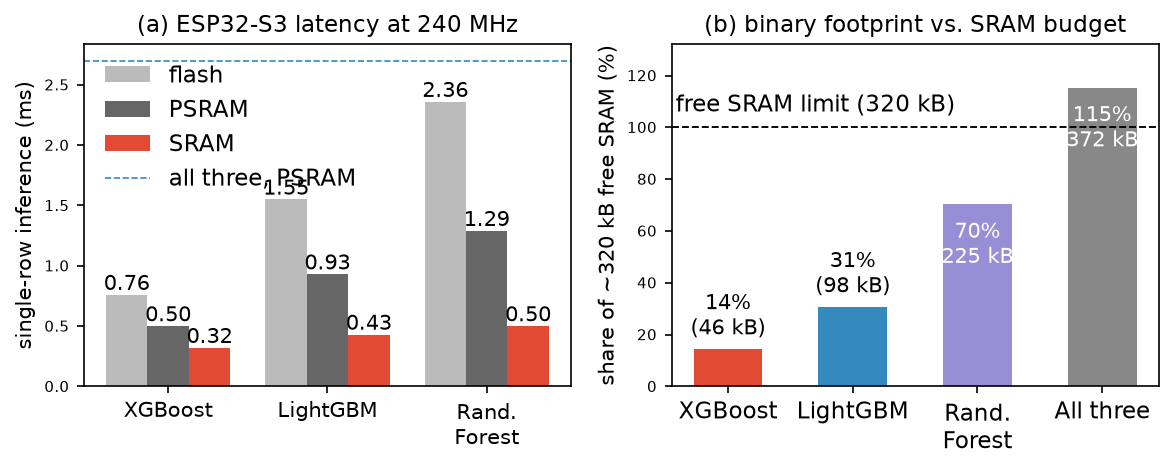
\includegraphics[width=0.9\textwidth]{fig_deploy.png}
\caption{Deployment trade-offs: (a) measured single-row inference time per model at 240 MHz with the binary in memory-mapped flash, PSRAM, or a single model in internal SRAM (dashed line: all three models from PSRAM); (b) per-model and combined binary footprint as a share of the ESP32-S3's roughly 320 kB of free internal SRAM --- each model fits, the combined 372 kB binary does not.}
\label{fig:deploy}
\end{figure}



\subsection{Replication on New Chemistries: NCA, NMC, and LFP Transfer Targets}
The transfer claim replicates on 60 Battery Archive NMC/NCA/LFP cells admitted under a pre-registered cleaning rule: with-SOH transfer spans 0.77--1.00 pooled AUC and drops to 0.36--0.91 outside the single-condition HNEI group, where full no-SOH transfer stays near 0.99 (audit figure and full table in the Supplementary Material).
\subsection{Operating-Condition Shift at Fixed Chemistry and Laboratory}
Holding out entire operating conditions at fixed chemistry and laboratory costs the sensor-only model while the SOH distance rule stays undisturbed (see Supplementary Material): no competing shortcut hides in temperature or C-rate.
\subsection{Key Findings}
\begin{itemize}
\item Within-distribution models are reliable (fold-mean AUC 0.90--0.96, Platt-calibrated) and run on-device in under a millisecond per SRAM-resident model.
\item Cross-dataset transfer collapses without SOH (Severson up to 0.90 with SOH to 0.53--0.75 without); an unfitted SOH distance rule matches the ensembles.
\item With-SOH numbers are diagnostic-proximity upper bounds: prognosis-only evaluation gives 0.838 [0.760, 0.991] on Severson and 0.73--0.99 on the new targets.
\item Dataset and laboratory shift govern the collapse at least as much as chemistry; narrow protocols transfer, diverse ones do not, with no temperature or C-rate shortcut in the available telemetry.
\item Source-fitted calibration and transferred thresholds do not survive shift; target recalibration repairs ECE but not ranking.
\end{itemize}

\section{Discussion, Analysis, and Novelty}

\subsection{The SOH Shortcut, Precisely Stated}
The evidence assembled above supports a precise statement. When a failure-risk model trained on one battery dataset is evaluated on another, its apparent transfer performance is dominated by the SOH coordinate; much of that dominance is definitional, because SOH enters the failure label itself, and the failure-definition ablation of Section~III-F measures how much: relabeling failure by voltage sag alone removes about a fifth of the with-SOH transfer advantage on Severson. What remains is a weak, real health-state signal; everything else the sensors measure is dataset-specific, and the factorial ablation shows no non-SOH feature group carries usable cross-dataset signal. The replication of Section~III-N extends each of these statements to data the pipeline never had access to when it was designed. ``SOH is a chemistry-specific lookup key,'' the earlier framing, claimed more than the design could identify; the defensible claim is that apparent cross-dataset transferability is largely a health-state shortcut whose size this paper measures with label-, feature-, and dataset-level controls.

\subsection{Implications for Battery Management Practitioners}
Four practical points follow:
\begin{itemize}
\item \textbf{1)} Within-chemistry, within-laboratory models from standard charge--discharge features are reliable (fold-mean AUC above 0.89, Platt-calibrated) and run on a \$12 microcontroller in under a millisecond per SRAM-resident model. Deploy them where the training distribution holds.
\item \textbf{2)} Do not transfer models across datasets on the strength of an AUC table. If SOH is available at the target, an unfitted threshold rule is the correct first baseline; if SOH is unavailable, expect chance-level performance unless the target protocol is as narrow as the source.
\item \textbf{3)} Quote risks from a coherent formulation: four independent classifiers can rank ``risk within 10 cycles'' above ``risk within 50 cycles,'' while the survival product of Section~II-G cannot.
\item \textbf{4)} Under shift, prefer raw or Platt-scaled scores, expect calibration to need labeled target data, and choose thresholds on source data with an explicit cost model --- then verify.
\end{itemize}

\subsection{Limitations}
The honesty of this paper has limits of its own. Oxford contributes five cells --- one with a single positive row --- at horizon-invariant 100-cycle logging resolution, so it is a pooled-detection target re-verified on Severson. CALCE contributes seven cells, so its leave-one-cell-out uncertainty is wide. The Battery Archive groups sharpen the chemistry claim but not the condition claim: SNL NCA/NMC span few conditions with as few as three cells each, and mostly-censored SNL LFP is supporting evidence. The export lacks per-cycle current and temperature; affected features are zero-imputed, conclusions rest on the common feature set, and the sensor collapse cannot rule out richer-telemetry signals. The small three-seed GRU convicts no architecture beyond this instance, was not re-evaluated on the Battery Archive targets, and might differ from pretrained, transformer, or state-space models. The hazard model scores post-failure rows like every formulation. Cost analysis fixes 20:1 with source-selected thresholds. Transfer remains one-directional (LCO sources); isolating chemistry needs same-laboratory cross-chemistry campaigns.

\section{Conclusion}
This study widened a multi-horizon failure-risk framework and found the widening demanded a validity analysis. Within dataset the framework is sound: fold-mean AUC 0.90--0.96 under cell-disjoint evaluation, a monotone discrete-time hazard formulation, and an about-372~kB deployment reproducing the training libraries to $1.1\times10^{-6}$ on a \$12 ESP32-S3.

Across datasets, the apparent transferability is mostly a State-of-Health shortcut. A distance-to-threshold rule on SOH alone reproduces the tuned ensembles' transfer performance; removing SOH collapses every model class toward or below chance; relabeling failure by voltage sag alone --- a criterion SOH does not define --- removes about a fifth of the with-SOH advantage; and same-chemistry cross-laboratory controls show the collapse is caused by dataset shift at least as much as by chemistry. The supported conclusion is deliberately narrower than ``SOH is chemistry-specific'': much of the observed cross-dataset discrimination is attributable to SOH, partly because SOH defines the failure criterion itself. Crucially, these statements replicate on 60 NMC, NCA and LFP cells from two further laboratories: with-SOH transfer spans 0.77--1.00 and drops to 0.36--0.91 without SOH outside the single-condition HNEI group (paired deltas 0.06--0.64) --- a pre-registered replication, not a post-hoc fit.

Calibration behaves as the validity story predicts: Platt preserves discrimination best at comparable calibration error, isotonic fails under shift, labeled-target recalibration repairs calibration error but not discrimination, and no score type yields a usable operating point without SOH. Evidence is carried by cell-level bootstrap intervals, with cycle-level tests demoted to a consistency check.

Future work, in order of directness: an SOH-free failure definition as the primary cross-dataset target; same-laboratory, cross-chemistry aging campaigns; learned dataset-invariant representations; cell-level hierarchical calibration; and multi-seed, multi-architecture sequence-model studies at generalizable scale.

\clearpage
\section*{Acknowledgment}
This work received no external funding. The authors declare no conflicts of interest. The source code, data, trained models, firmware, and validation pipeline are publicly available at \url{https://github.com/touhidsiddiqueeraj-bit/Multi-Horizon-Hazard-Models-for-Battery-Failure-Prediction}.

\raggedbottom
\begin{thebibliography}{99}
\bibitem{meng2019review} H. Meng and Y. Li, ``A review on prognostics and health management (PHM) methods of lithium-ion batteries,'' \emph{Renew. Sustain. Energy Rev.}, vol. 116, Art. no. 109405, 2019.
\bibitem{roman2021machine} D. Roman, S. Saxena, V. Robu, et al., ``Machine learning pipeline for battery state-of-health estimation,'' \emph{Nat. Mach. Intell.}, vol. 3, no. 4, pp. 447--456, 2021.
\bibitem{sulzer2021challenge} V. Sulzer, P. Mohtat, A. Aitio, et al., ``The challenge and opportunity of battery lifetime prediction from field data,'' \emph{Joule}, vol. 5, no. 8, pp. 1934--1955, 2021.
\bibitem{breiman2001random} L. Breiman, ``Random forests,'' \emph{Mach. Learn.}, vol. 45, no. 1, pp. 5--32, 2001.
\bibitem{chen2016xgboost} T. Chen and C. Guestrin, ``XGBoost: A scalable tree boosting system,'' in \emph{Proc. ACM SIGKDD}, 2016, pp. 785--794.
\bibitem{ke2017lightgbm} G. Ke, Q. Meng, T. Finley, et al., ``LightGBM: A highly efficient gradient boosting decision tree,'' in \emph{Proc. NeurIPS}, vol. 30, 2017, pp. 3146--3154.
\bibitem{shikdar2026learning} T. A. Shikdar and H. Laaksonen, ``Learning when not to use a battery: Multihorizon failure intelligence,'' \emph{Int. Trans. Electr. Energy Syst.}, vol. 36, Art. no. 6000810, 2026.
\bibitem{sahoo2022transfer} S. Sahoo, K. S. Hariharan, S. Agarwal, et al., ``Transfer learning based generalized framework for state of health estimation of Li-ion cells,'' \emph{Sci. Rep.}, vol. 12, Art. no. 13173, 2022.
\bibitem{lu2023deep} J. Lu, R. Xiong, J. Tian, C. Wang, and F. Sun, ``Deep learning to estimate lithium-ion battery state of health without additional degradation experiments,'' \emph{Nat. Commun.}, vol. 14, Art. no. 2760, 2023.
\bibitem{platt1999probabilistic} J. C. Platt, ``Probabilistic outputs for support vector machines and comparisons to regularized likelihood methods,'' in \emph{Adv. Large Margin Classifiers}, MIT Press, 1999, pp. 61--74.
\bibitem{zadrozny2002transforming} B. Zadrozny and C. Elkan, ``Transforming classifier scores into accurate multiclass probability estimates,'' in \emph{Proc. ACM SIGKDD}, 2002, pp. 694--699.
\bibitem{niculescu2005predicting} A. Niculescu-Mizil and R. Caruana, ``Predicting good probabilities with supervised learning,'' in \emph{Proc. ICML}, 2005, pp. 625--632.
\bibitem{huang2020experimental} L. Huang, J. Zhao, B. Zhu, H. Chen, and S. K. L. M. v. Broucke, ``An experimental investigation of calibration techniques for imbalanced data,'' \emph{IEEE Access}, vol. 8, pp. 127343--127352, 2020.
\bibitem{shikdar2026robustness} T. A. Shikdar and H. Laaksonen, ``How far does the model hold? Robustness of multihorizon battery failure intelligence under realistic operating conditions,'' submitted for publication, 2026.
\bibitem{lundberg2020from} S. M. Lundberg, G. G. Erion, H. Chen, et al., ``From local explanations to global understanding with explainable AI for trees,'' \emph{Nat. Mach. Intell.}, vol. 2, no. 1, pp. 56--67, 2020.
\bibitem{grzesik2024combining} P. Grzesik and D. Mrozek, ``Combining machine learning and edge computing: Opportunities, challenges, platforms, frameworks, and use cases,'' \emph{Electronics}, vol. 13, no. 3, Art. no. 640, 2024.
\bibitem{gupta2023online} C. Gupta and A. Ramdas, ``Online Platt scaling with calibeating,'' in \emph{Proc. ICML}, PMLR 202, 2023, pp. 12182--12204.
\bibitem{saha2007battery} B. Saha and K. Goebel, ``Battery data set,'' NASA Ames Prognostics Data Repository, 2007.
\bibitem{calce2023battery} CALCE Battery Research Group, ``Battery aging datasets,'' Univ. Maryland, 2023.
\bibitem{birkl2017oxford} C. R. Birkl and D. A. Howey, ``Oxford battery degradation dataset 1,'' Univ. Oxford, 2017.
\bibitem{severson2019data} K. A. Severson, P. M. Attia, N. Jin, et al., ``Data-driven prediction of battery cycle life before capacity degradation,'' \emph{Nature Energy}, vol. 4, pp. 383--391, 2019.
\bibitem{attia2020closedloop} P. M. Attia, A. Grover, N. Jin, et al., ``Closed-loop optimization of fast-charging protocols for batteries with machine learning,'' \emph{Nature}, vol. 578, no. 7795, pp. 397--402, 2020.
\bibitem{batteryarchive2023} Battery Archive, ``Open battery degradation testing data,'' 2023. [Online]. Available: \url{https://batteryarchive.org}. Consolidated cell cycling records from the Hawaii Natural Energy Institute and Sandia National Laboratories.
\bibitem{preger2020degradation} Y. Preger, H. C. Barkholtz, A. Fresquez, et al., ``Degradation of commercial lithium-ion cells as a function of chemistry and cycling conditions,'' \emph{J. Electrochem. Soc.}, vol. 167, no. 12, Art. no. 120532, 2020.
\bibitem{delong1988comparing} E. R. DeLong, D. M. DeLong, and D. L. Clarke-Pearson, ``Comparing the areas under two or more correlated receiver operating characteristic curves: A nonparametric approach,'' \emph{Biometrics}, vol. 44, no. 3, pp. 837--845, 1988.
\end{thebibliography}
\end{document}
